\documentclass[journal,onecolumn]{IEEEtran}

\usepackage[utf8]{inputenc}
\usepackage[T1]{fontenc}
\usepackage[brazil]{babel}
\usepackage{amsmath,amssymb,amsfonts}
\usepackage{graphicx}
\usepackage{booktabs}
\usepackage{cite}
\usepackage{float}
\usepackage{hyperref}
\hypersetup{
    colorlinks=true,
    linkcolor=blue,
    filecolor=magenta,
    urlcolor=blue,
}

\begin{document}

\title{Relatório de Inteligência Artificial Computacional: Redes Neurais Artificiais}

\author{Tiago Silveira Taumaturgo (2410518),
        Vinicius Lira Cavalcante (2314980), \\
        William Wallace Sena Nogueira (2310284)
\thanks{Trabalho apresentado à disciplina de Inteligência Artificial Computacional da Universidade de Fortaleza (UNIFOR). Professor: Msc. Paulo Cirillo Souza Barbosa.}}
\markboth{UNIFOR - Centro de Ciências Tecnológicas - CCT}{}

\maketitle

\begin{abstract}
Este relatório apresenta a implementação e a análise de redes neurais artificiais aplicadas a dois problemas supervisionados. A primeira etapa aborda a classificação binária do conjunto \textit{spiral\_d}, com estudo de underfitting e overfitting em Perceptron de Múltiplas Camadas (MLP) e comparação estatística entre Perceptron Simples, ADALINE, MLP e RBF. A segunda etapa trata do reconhecimento facial multiclasse com 20 pessoas, a partir do redimensionamento das imagens para $30\times30$ pixels e codificação \textit{one-hot} bipolar. O código-fonte completo utilizado neste trabalho está disponível em: \href{https://github.com/tiagostmg/iac}{https://github.com/tiagostmg/iac}.
\end{abstract}

\begin{IEEEkeywords}
Inteligência Artificial Computacional, Redes Neurais Artificiais, Perceptron, ADALINE, MLP, RBF, Reconhecimento Facial.
\end{IEEEkeywords}

\section{Introdução}
\IEEEPARstart{E}{ste} trabalho tem como objetivo validar a implementação de modelos neurais lineares e não lineares em dois cenários distintos. Na etapa 1, o problema consiste em classificar duas espirais entrelaçadas, um caso clássico de separação não linear. Na etapa 2, o objetivo é reconhecer 20 indivíduos distintos em um conjunto de 640 imagens faciais.

O código-fonte utilizado na construção deste relatório encontra-se no repositório do projeto e, para esta versão do documento, foram considerados principalmente os artefatos gerados por \texttt{main\_pt1\_edit\_sem\_rfb.py}, \texttt{main\_pt1\_edit.py} e \texttt{main pt2.py}. Na etapa 1, os resultados consolidados também incluem a RBF para comparação estatística global entre arquiteturas.

\section{Metodologia}

\subsection{Etapa 1: Classificação Binária no \textit{spiral\_d}}
O conjunto \textit{spiral\_d} foi lido a partir de arquivo CSV, com duas variáveis de entrada e um rótulo binário por amostra. Os rótulos foram convertidos para codificação bipolar $\{-1,+1\}$, e os dados foram particionados em 80\% para treinamento e 20\% para teste a cada rodada. A normalização foi realizada por reescalonamento bipolar com base apenas no conjunto de treinamento.

Os modelos avaliados nesta etapa foram:
\begin{itemize}
    \item \textbf{Perceptron Simples:} taxa de aprendizagem $0{,}01$ e máximo de 300 épocas.
    \item \textbf{ADALINE:} taxa de aprendizagem $0{,}01$, precisão $10^{-4}$ e máximo de 300 épocas.
    \item \textbf{MLP:} topologia base $[10,6]$, taxa de aprendizagem $0{,}02$, precisão $10^{-4}$ e máximo de 400 épocas.
\end{itemize}

Para investigar underfitting e overfitting na MLP, foram testadas três topologias:
\begin{itemize}
    \item \textbf{Underfitting:} $[2]$, 200 épocas.
    \item \textbf{Ajuste intermediário:} $[10,6]$, 400 épocas.
    \item \textbf{Overfitting:} $[24,18,12]$, 500 épocas.
\end{itemize}

A validação dos modelos foi feita por simulação de Monte Carlo com $R=500$ rodadas. Em cada rodada foram calculadas as métricas acurácia, sensibilidade, especificidade, precisão e $F_{1}$-score. Para as rodadas de maior e menor acurácia, foram salvas também as curvas de aprendizado e as matrizes de confusão.

\subsection{Etapa 2: Reconhecimento Facial Multiclasse}
Na segunda etapa foi utilizado o conjunto \texttt{RecFac}, composto por 640 imagens de faces distribuídas em 20 classes. Cada imagem original foi convertida para tons de cinza, redimensionada para $30\times30$ pixels e vetorizada, resultando em $900$ atributos por amostra. A matriz de entrada foi organizada no formato $X \in \mathbb{R}^{900\times640}$ e a matriz de saídas no formato bipolar \textit{one-hot}, com $Y \in \mathbb{R}^{20\times640}$.

Os hiperparâmetros escolhidos foram:
\begin{itemize}
    \item \textbf{ADALINE:} taxa de aprendizagem $0{,}01$, precisão $10^{-5}$ e máximo de 500 épocas.
    \item \textbf{MLP:} uma camada oculta com 50 neurônios, taxa de aprendizagem $0{,}1$, precisão $10^{-5}$ e máximo de 500 épocas.
    \item \textbf{RBF:} 30 neurônios na camada radial, taxa de aprendizagem $0{,}1$, precisão $10^{-5}$ e máximo de 300 épocas.
\end{itemize}

Para os tópicos de inspeção visual do enunciado, foram executadas 10 rodadas de Monte Carlo com particionamento 80/20, registrando a melhor e a pior acurácia de cada modelo, juntamente com suas curvas de aprendizado e matrizes de confusão. Para a análise estatística final, foram utilizadas 100 rodadas, calculando-se média, desvio-padrão, maior valor e menor valor da acurácia.

\section{Resultados e Discussão}

\subsection{Etapa 1: Espirais Bidimensionais}
A visualização inicial do conjunto \textit{spiral\_d} mostra duas classes com forte interdependência geométrica e separação nitidamente não linear, o que já antecipa a limitação dos modelos estritamente lineares.

\begin{figure}[H]
    \centering
    
\includegraphics[width=0.72\linewidth]{\detokenize{../redes_neurais/outputs pt1 edit sem rfb/spiral_scatter.png}}
    \caption{Visualização inicial do conjunto \textit{spiral\_d}.}
\end{figure}

O estudo de complexidade da MLP confirmou esse comportamento. Na configuração subdimensionada, a curva de aprendizado decresce lentamente e estabiliza em patamar mais alto de erro, evidenciando capacidade insuficiente para representar a estrutura espiral. Já a configuração intermediária reduz o EQM de forma rápida e estável, enquanto a topologia superdimensionada continua reduzindo o erro por mais épocas, com maior flexibilidade do modelo.

\begin{figure}[H]
    \centering
    \begin{minipage}{0.32\textwidth}
        \centering
        
\includegraphics[width=\linewidth]{\detokenize{../redes_neurais/outputs pt1 edit sem rfb/etapa1_mlp_underfitting_curva.png}}
        \caption{MLP com underfitting.}
    \end{minipage}\hfill
    \begin{minipage}{0.32\textwidth}
        \centering
        
\includegraphics[width=\linewidth]{\detokenize{../redes_neurais/outputs pt1 edit sem rfb/etapa1_mlp_ajuste_intermediario_curva.png}}
        \caption{MLP com ajuste intermediário.}
    \end{minipage}\hfill
    \begin{minipage}{0.32\textwidth}
        \centering
        
\includegraphics[width=\linewidth]{\detokenize{../redes_neurais/outputs pt1 edit sem rfb/etapa1_mlp_overfitting_curva.png}}
        \caption{MLP com maior complexidade.}
    \end{minipage}
\end{figure}

Na validação por Monte Carlo, a diferença entre os modelos ficou evidente. O boxplot de acurácia indica que o Perceptron Simples apresentou a pior distribuição e grande dispersão, o ADALINE obteve melhora moderada, mas continuou limitado pela linearidade, e a MLP concentrou os resultados mais altos e mais estáveis. Isso é coerente com a natureza do problema: as espirais exigem fronteiras não lineares, o que favorece a MLP.

\begin{figure}[H]
    \centering
    
\includegraphics[width=0.78\linewidth]{\detokenize{../redes_neurais/outputs pt1 edit/etapa1_boxplot_accuracy.png}}
    \caption{Distribuição da acurácia na etapa 1 ao longo das rodadas de Monte Carlo.}
\end{figure}

Ao final da rotina de geração de relatórios, boxplots e matrizes finais, foram obtidos os resumos estatísticos das 500 rodadas de Monte Carlo para cada métrica. As Tabelas I a V consolidam exatamente esses resultados.

\begin{table}[H]
\renewcommand{\arraystretch}{1.2}
\caption{ETAPA 1: RESUMO DA ACURÁCIA}
\centering
\begin{tabular}{lcccc}
\hline
\textbf{Modelo} & \textbf{Média} & \textbf{Desvio} & \textbf{Máx} & \textbf{Mín} \\ \hline
Perceptron & 0,7239 & 0,0923 & 0,8750 & 0,2714 \\
ADALINE & 0,7868 & 0,0302 & 0,8714 & 0,6929 \\
MLP & 0,9899 & 0,0073 & 1,0000 & 0,9571 \\
RBF & 0,9517 & 0,0315 & 0,9964 & 0,7607 \\ \hline
\end{tabular}
\end{table}

\begin{table}[H]
\renewcommand{\arraystretch}{1.2}
\caption{ETAPA 1: RESUMO DA SENSIBILIDADE}
\centering
\begin{tabular}{lcccc}
\hline
\textbf{Modelo} & \textbf{Média} & \textbf{Desvio} & \textbf{Máx} & \textbf{Mín} \\ \hline
Perceptron & 0,8069 & 0,2043 & 1,0000 & 0,0000 \\
ADALINE & 0,8835 & 0,0473 & 1,0000 & 0,7586 \\
MLP & 0,9944 & 0,0057 & 1,0000 & 0,9650 \\
RBF & 0,9730 & 0,0250 & 1,0000 & 0,8526 \\ \hline
\end{tabular}
\end{table}

\begin{table}[H]
\renewcommand{\arraystretch}{1.2}
\caption{ETAPA 1: RESUMO DA ESPECIFICIDADE}
\centering
\begin{tabular}{lcccc}
\hline
\textbf{Modelo} & \textbf{Média} & \textbf{Desvio} & \textbf{Máx} & \textbf{Mín} \\ \hline
Perceptron & 0,5183 & 0,2670 & 1,0000 & 0,0000 \\
ADALINE & 0,5466 & 0,0567 & 0,7160 & 0,3882 \\
MLP & 0,9791 & 0,0222 & 1,0000 & 0,8537 \\
RBF & 0,8986 & 0,0824 & 1,0000 & 0,4861 \\ \hline
\end{tabular}
\end{table}

\begin{table}[H]
\renewcommand{\arraystretch}{1.2}
\caption{ETAPA 1: RESUMO DA PRECISÃO}
\centering
\begin{tabular}{lcccc}
\hline
\textbf{Modelo} & \textbf{Média} & \textbf{Desvio} & \textbf{Máx} & \textbf{Mín} \\ \hline
Perceptron & 0,8127 & 0,1122 & 1,0000 & 0,0000 \\
ADALINE & 0,8296 & 0,0239 & 0,8905 & 0,7626 \\
MLP & 0,9916 & 0,0090 & 1,0000 & 0,9429 \\
RBF & 0,9607 & 0,0310 & 1,0000 & 0,7877 \\ \hline
\end{tabular}
\end{table}

\begin{table}[H]
\renewcommand{\arraystretch}{1.2}
\caption{ETAPA 1: RESUMO DO $F_{1}$-SCORE}
\centering
\begin{tabular}{lcccc}
\hline
\textbf{Modelo} & \textbf{Média} & \textbf{Desvio} & \textbf{Máx} & \textbf{Mín} \\ \hline
Perceptron & 0,7905 & 0,1288 & 0,9241 & 0,0000 \\
ADALINE & 0,8548 & 0,0239 & 0,9193 & 0,7713 \\
MLP & 0,9930 & 0,0052 & 1,0000 & 0,9706 \\
RBF & 0,9664 & 0,0218 & 0,9975 & 0,8329 \\ \hline
\end{tabular}
\end{table}

As matrizes de confusão de melhor caso reforçam esse diagnóstico. Enquanto o ADALINE ainda mantém quantidade relevante de falsos positivos sobre a classe $-1$, a MLP atinge separação praticamente perfeita no melhor cenário observado, evidenciando ganho expressivo de representação.

\begin{figure}[H]
    \centering
    \begin{minipage}{0.46\textwidth}
        \centering
        
\includegraphics[width=\linewidth]{\detokenize{../redes_neurais/outputs pt1 edit/etapa1_adaline_melhor_matriz.png}}
        \caption{ADALINE: melhor matriz de confusão.}
    \end{minipage}\hfill
    \begin{minipage}{0.46\textwidth}
        \centering
        
\includegraphics[width=\linewidth]{\detokenize{../redes_neurais/outputs pt1 edit/etapa1_mlp_melhor_matriz.png}}
        \caption{MLP: melhor matriz de confusão.}
    \end{minipage}
\end{figure}

\textbf{Análise técnica:} a etapa 1 funcionou como validador das implementações. Os resultados visuais e estatísticos mostram que os modelos lineares não conseguem capturar adequadamente o traçado das espirais, mesmo quando treinados por várias rodadas. O Perceptron teve acurácia média de apenas 72,39\% e especificidade média de 51,83\%, evidenciando grande dificuldade em modelar corretamente a classe negativa. O ADALINE melhorou a estabilidade e elevou a acurácia média para 78,68\%, mas continuou com especificidade limitada. Entre os modelos não lineares, a RBF já apresentou desempenho elevado, com 95,17\% de acurácia média, porém a MLP foi a arquitetura de maior destaque, alcançando 98,99\% de acurácia média, 99,44\% de sensibilidade e 99,30\% de $F_{1}$-score. Esses números confirmam que a escolha de uma topologia oculta moderada foi suficiente para representar a não linearidade do problema com excelente generalização.

\subsection{Etapa 2: Reconhecimento Facial}
A Figura 6 apresenta um exemplo de imagem facial após o redimensionamento para $30\times30$, escolha que equilibra redução de dimensionalidade com preservação dos traços principais de face.

\begin{figure}[H]
    \centering
    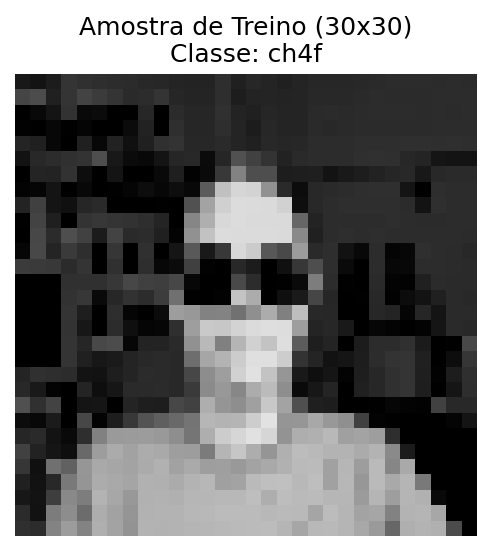
\includegraphics[width=0.32\linewidth]{../redes_neurais/outputs_pt2/amostra_redimensionada_30x30.png}
    \caption{Exemplo de amostra redimensionada para $30\times30$ pixels.}
\end{figure}

Os resultados de 100 rodadas de Monte Carlo estão sumarizados na Tabela VI. Observa-se que ADALINE e MLP alcançaram acurácia média acima de 97\%, com vantagem para a MLP tanto na média quanto na estabilidade. Em contraste, a RBF apresentou desempenho bastante inferior neste problema específico, com média próxima de 21\%, indicando forte inadequação da configuração adotada para o reconhecimento facial após o redimensionamento das imagens.

\begin{table}[H]
\renewcommand{\arraystretch}{1.3}
\caption{RESULTADOS DA ETAPA 2 PARA ACURÁCIA ($R=100$)}
\centering
\begin{tabular}{lcccc}
\hline
\textbf{Modelo} & \textbf{Média} & \textbf{Desvio-Padrão} & \textbf{Maior Valor} & \textbf{Menor Valor} \\ \hline
ADALINE & 0,9723 & 0,0148 & 1,0000 & 0,9375 \\
MLP & 0,9780 & 0,0138 & 1,0000 & 0,9297 \\
RBF & 0,2103 & 0,0531 & 0,3828 & 0,1250 \\ \hline
\end{tabular}
\end{table}

O boxplot das 100 rodadas mostra distribuições muito próximas para ADALINE e MLP, mas a rede MLP aparece com mediana ligeiramente superior. A RBF, por outro lado, ficou concentrada em patamar muito baixo de desempenho, evidenciando alta dificuldade para discriminar corretamente as 20 identidades com a parametrização utilizada. Isso indica que, mesmo após forte redução de dimensionalidade, a presença de uma camada oculta densa na MLP ainda oferece um ganho consistente, enquanto a formulação radial empregada não conseguiu generalizar adequadamente.

\begin{figure}[H]
    \centering
    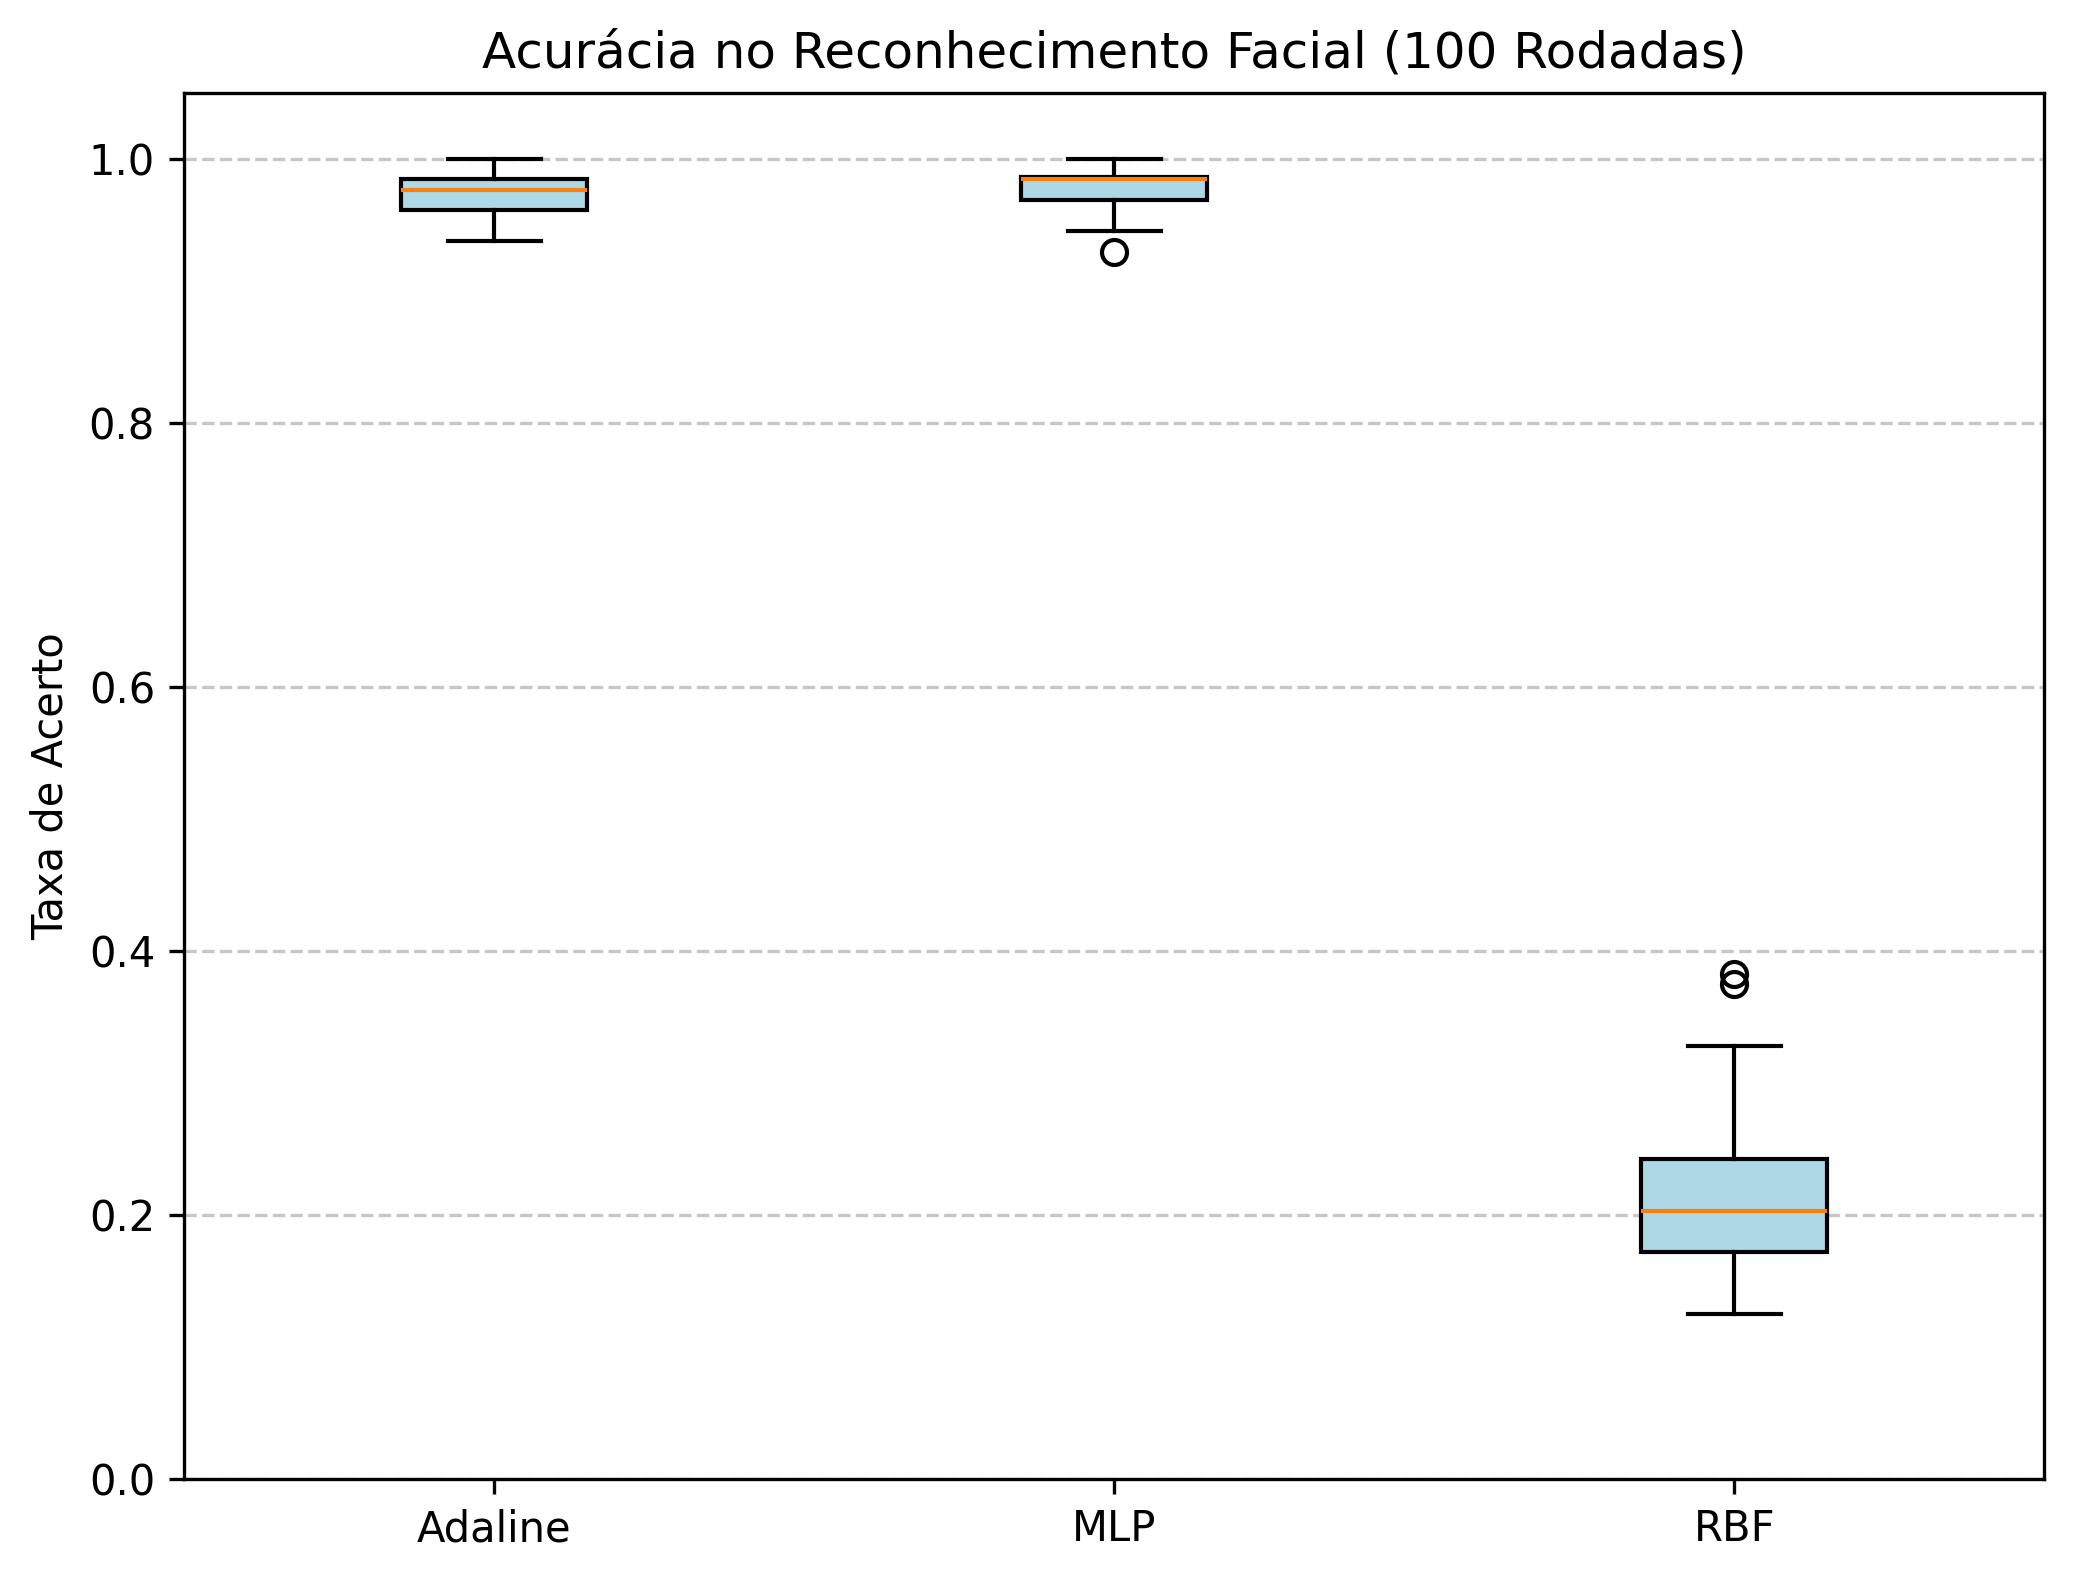
\includegraphics[width=0.78\linewidth]{../redes_neurais/outputs_pt2/etapa2_boxplot_topico7.png}
    \caption{Distribuição da acurácia na etapa 2.}
\end{figure}

Nas matrizes de confusão de melhor caso, ADALINE e MLP apresentam diagonal principal dominante, com pouquíssimos erros fora dela. Já nos piores casos, os erros continuam esparsos e parecem concentrar-se em identidades específicas, sugerindo que determinadas faces compartilham padrões visuais semelhantes após o redimensionamento. Em particular, aparecem trocas pontuais envolvendo classes como \textit{glikman}, \textit{karyadi}, \textit{bpm}, \textit{mitchell} e \textit{tammo}, mas sem colapso global desses classificadores. A RBF exibe um comportamento bem diferente: mesmo em seu melhor caso, a matriz de confusão revela dispersão intensa das predições entre muitas classes, sinalizando baixa capacidade de separação no espaço transformado.

\begin{figure}[H]
    \centering
    \begin{minipage}{0.46\textwidth}
        \centering
        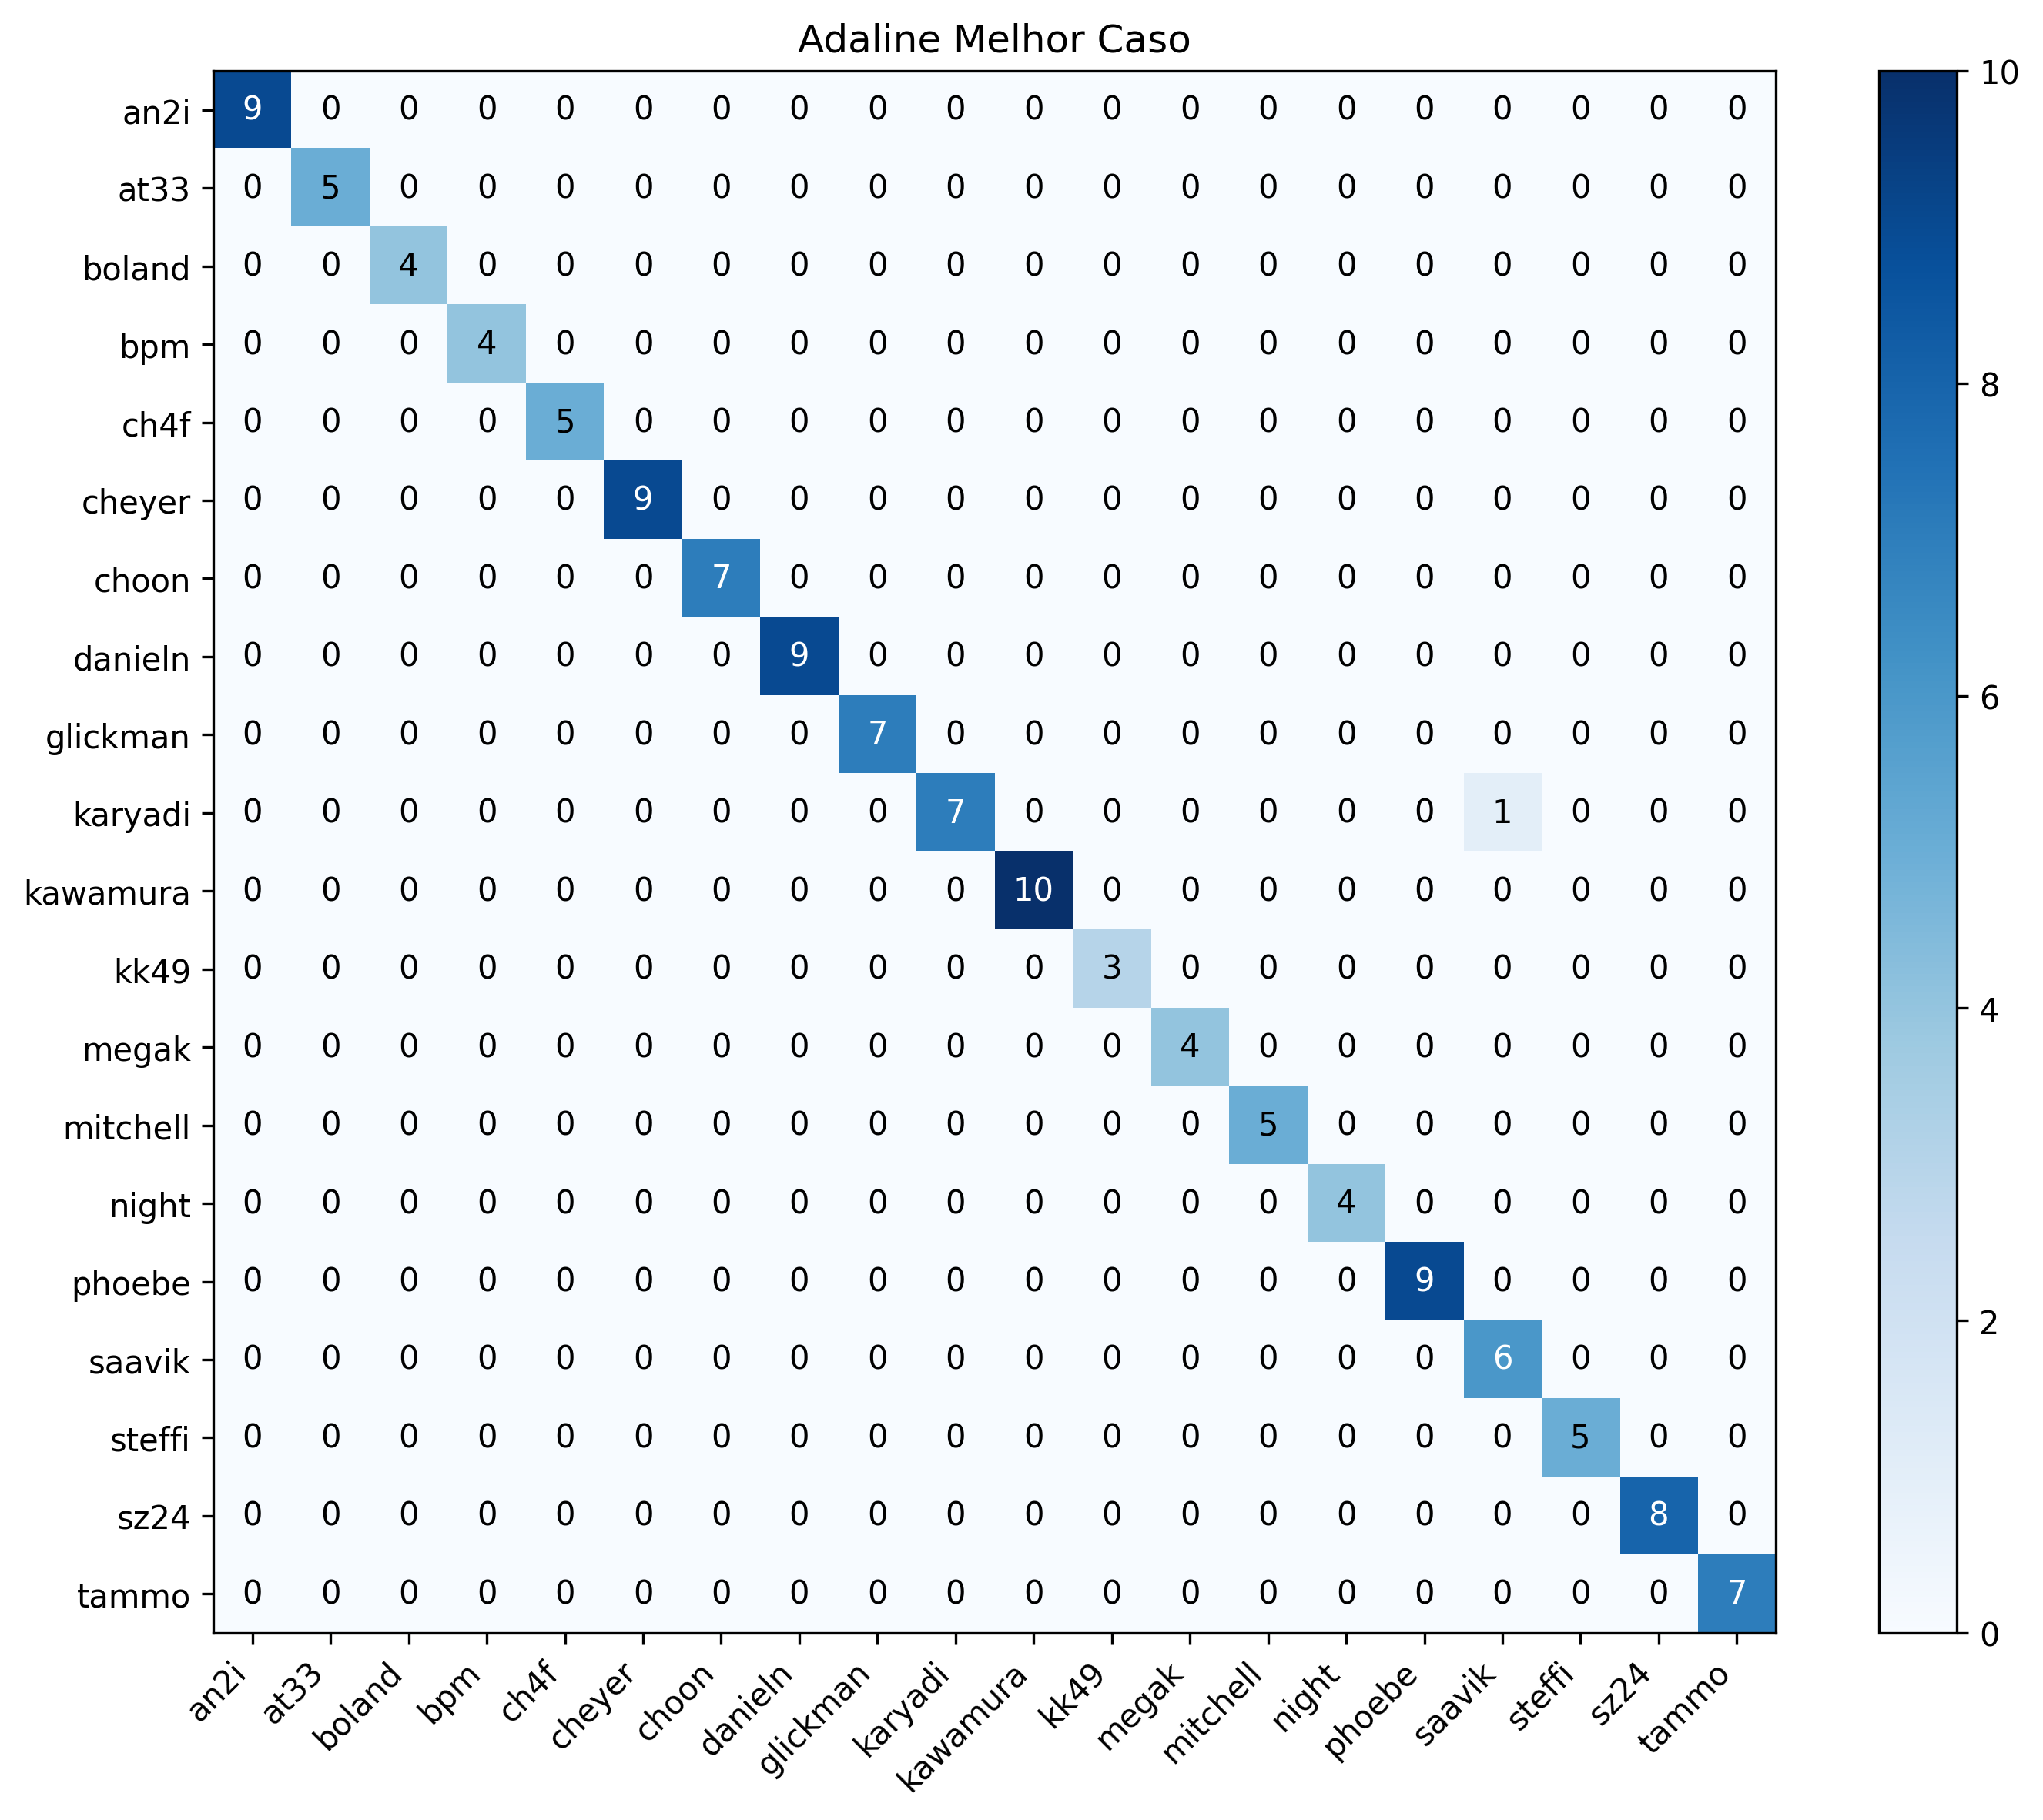
\includegraphics[width=\linewidth]{../redes_neurais/outputs_pt2/etapa2_adaline_melhor_matriz.png}
        \caption{ADALINE: melhor caso.}
    \end{minipage}\hfill
    \begin{minipage}{0.46\textwidth}
        \centering
        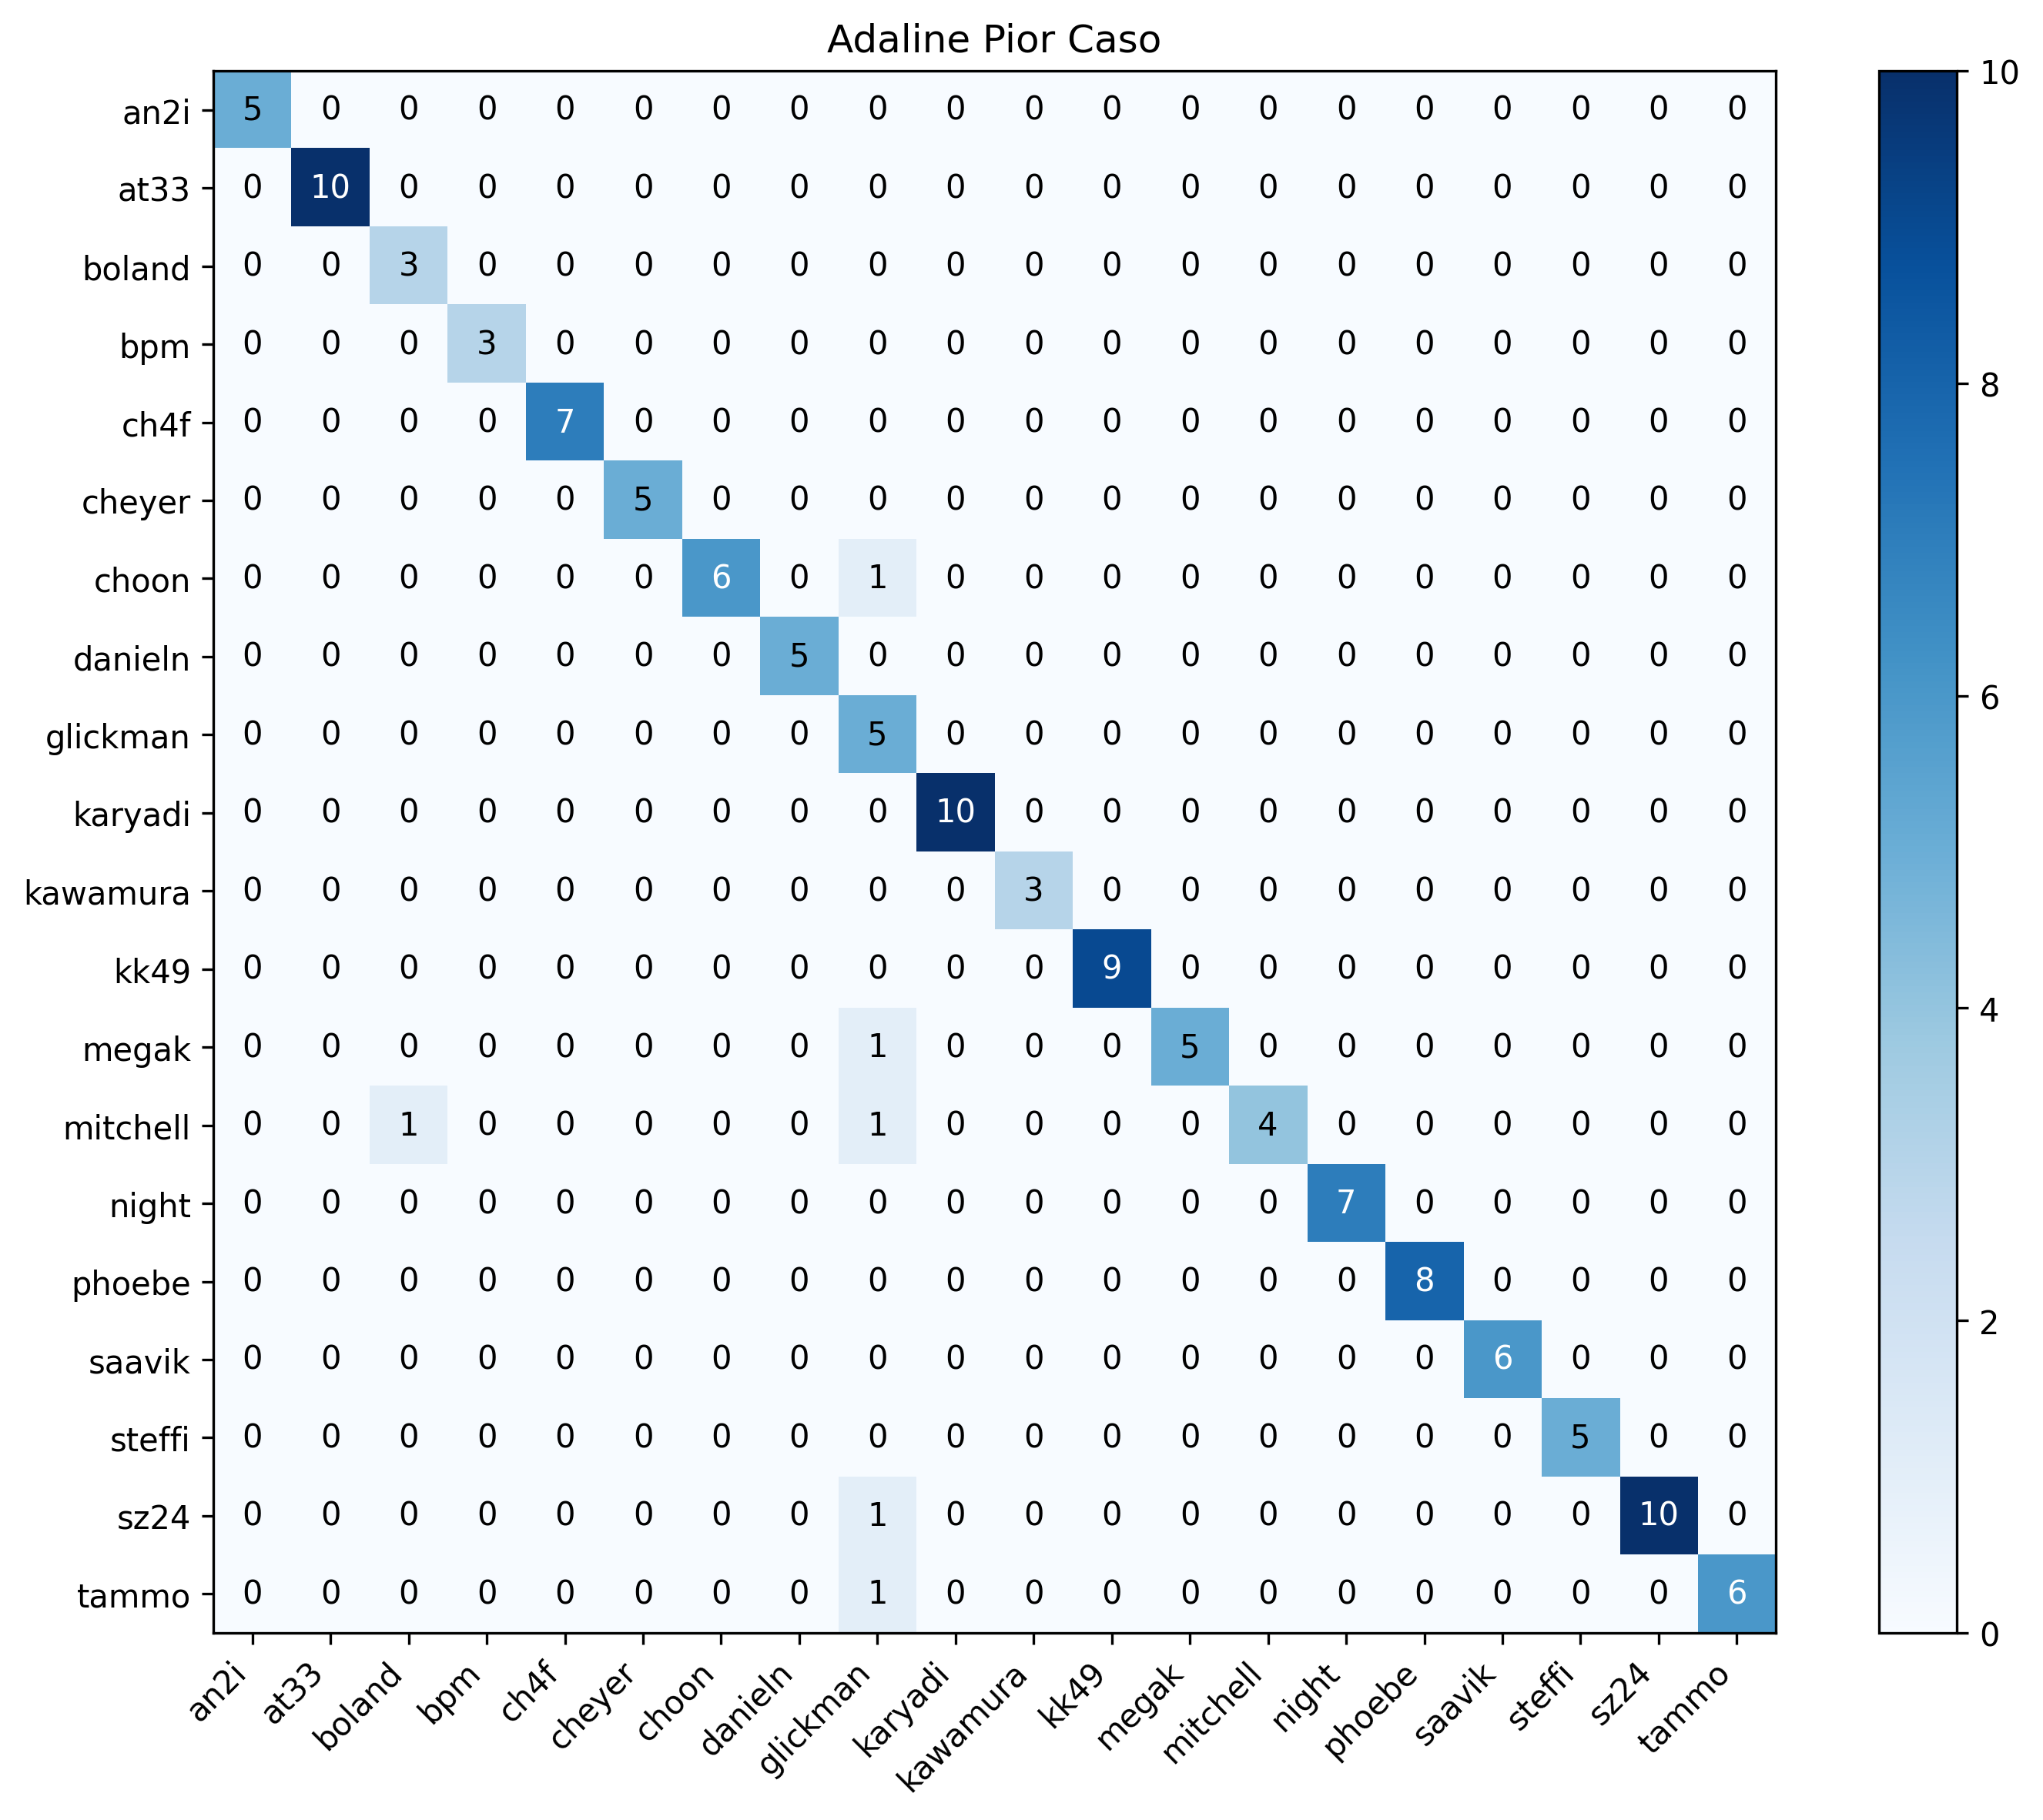
\includegraphics[width=\linewidth]{../redes_neurais/outputs_pt2/etapa2_adaline_pior_matriz.png}
        \caption{ADALINE: pior caso.}
    \end{minipage}
\end{figure}

\begin{figure}[H]
    \centering
    \begin{minipage}{0.46\textwidth}
        \centering
        
\includegraphics[width=\linewidth]{../redes_neurais/outputs_pt2/etapa2_mlp_melhor_matriz.png}
        \caption{MLP: melhor caso.}
    \end{minipage}\hfill
    \begin{minipage}{0.46\textwidth}
        \centering
        
\includegraphics[width=\linewidth]{../redes_neurais/outputs_pt2/etapa2_mlp_pior_matriz.png}
        \caption{MLP: pior caso.}
    \end{minipage}
\end{figure}

\begin{figure}[H]
    \centering
    \begin{minipage}{0.46\textwidth}
        \centering
        
\includegraphics[width=\linewidth]{../redes_neurais/outputs_pt2/etapa2_rbf_melhor_matriz.png}
        \caption{RBF: melhor caso.}
    \end{minipage}\hfill
    \begin{minipage}{0.46\textwidth}
        \centering
        
\includegraphics[width=\linewidth]{../redes_neurais/outputs_pt2/etapa2_rbf_pior_matriz.png}
        \caption{RBF: pior caso.}
    \end{minipage}
\end{figure}

\textbf{Análise técnica:} os resultados da etapa 2 mostram que o problema de reconhecimento facial, embora multiclasse, ficou bem condicionado após o redimensionamento para $30\times30$ para alguns modelos, mas não para todos. O ADALINE já obteve excelente desempenho, o que sugere que boa parte das classes tornou-se aproximadamente separável no espaço de atributos adotado. A MLP superou levemente esse resultado ao incorporar uma camada oculta com 50 neurônios, preservando alta taxa de acerto e baixa variabilidade. Em contraste, a RBF apresentou acurácia média de apenas 21,03\%, com desvio-padrão de 5,31\%, resultado muito distante dos demais modelos. Isso sugere que a escolha de 30 centros radiais e o modo de ajuste utilizado não foram suficientes para representar a variabilidade intra-classe e a separação entre as 20 pessoas. Em outras palavras, a não linearidade adicional da MLP foi útil, mas a formulação radial empregada nesta configuração não conseguiu transformar essa flexibilidade em generalização eficaz.

\section{Conclusões}
Os experimentos confirmam a adequação das implementações neurais nas duas etapas propostas. No problema \textit{spiral\_d}, os modelos lineares mostraram limitações claras diante de uma fronteira altamente não linear, enquanto a MLP apresentou o melhor compromisso entre capacidade de representação e estabilidade estatística. O estudo de underfitting e overfitting foi importante para mostrar que a escolha da topologia interfere diretamente na qualidade da convergência.

No reconhecimento facial multiclasse, a estratégia de redimensionar as imagens para $30\times30$ pixels e codificar as saídas em \textit{one-hot} bipolar produziu resultados muito fortes para ADALINE e MLP, ambos com acurácia média superior a 97\%, e ligeira vantagem para a MLP. A RBF, por sua vez, teve desempenho bastante inferior nessa etapa, mostrando que nem toda arquitetura não linear responde da mesma forma ao problema quando submetida à mesma redução de dimensionalidade. Assim, conclui-se que a arquitetura multicamada foi a mais consistente no conjunto de experimentos analisados.

\begin{thebibliography}{1}
\bibitem{roteiro}
P. C. S. Barbosa, ``Trabalho Computacional AV2: Redes Neurais Artificiais,'' UNIFOR, 2026.
\end{thebibliography}

\end{document}
